\begin{figure}[h!]
    \begin{center}
    \caption{Effects on Primary Care Related Infrastructure and Human Resources: N. of Health Facilities with:}\label{fig:12}
    \begin{subfigure}{0.32\textwidth}
        \centering
        \caption{\scriptsize Ambulatory Service and ACS Teams}\label{fig:12a}
        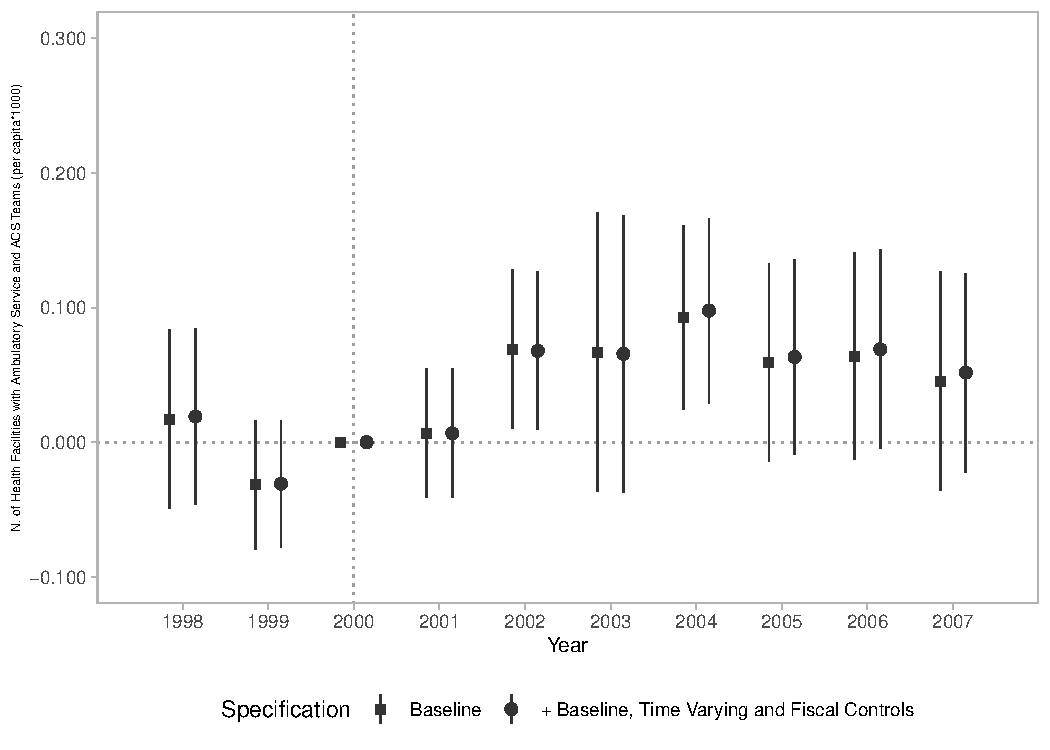
\includegraphics[width=\textwidth]{plots/sia_ncnes_acs_pcapita_dist_ec29_baseline_dist_ec29_baseline_12.pdf}
    \end{subfigure}
    \begin{subfigure}{0.32\textwidth}
        \caption{\scriptsize Ambulatory Service and Community Doctors}\label{fig:12b}
        \centering
        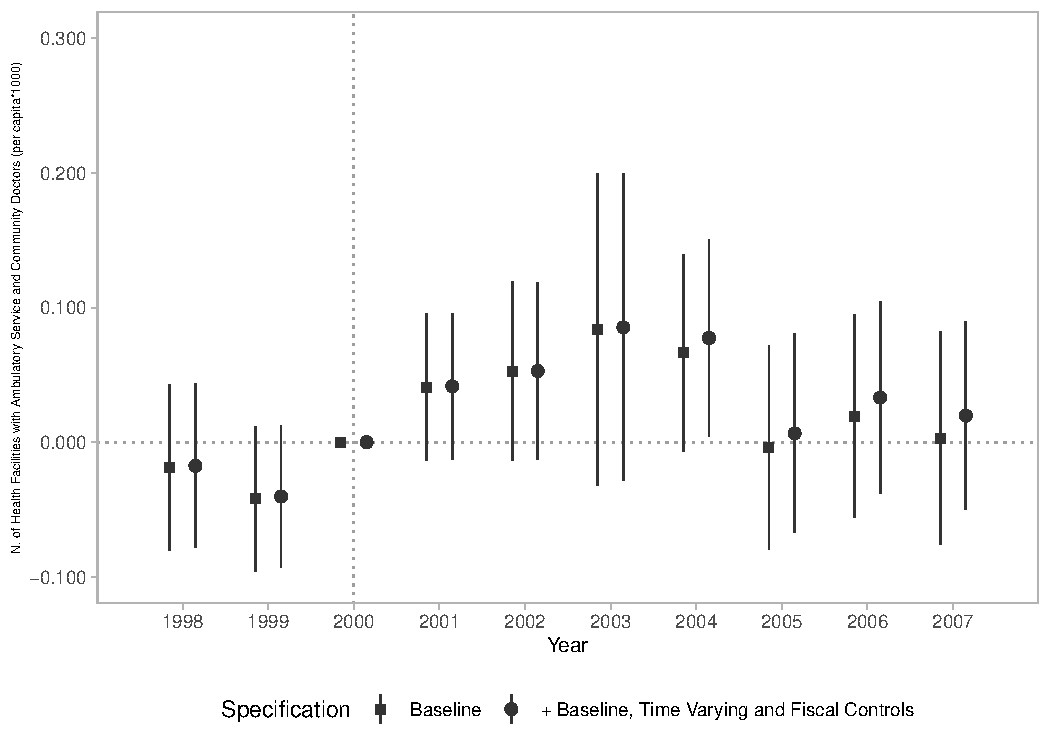
\includegraphics[width=\textwidth]{plots/sia_ncnes_medcom_pcapita_dist_ec29_baseline_dist_ec29_baseline_12.pdf}
    \end{subfigure}
    \begin{subfigure}{0.32\textwidth}
        \centering
        \caption{\scriptsize Ambulatory Service and ACS Nurses}\label{fig:12c}
        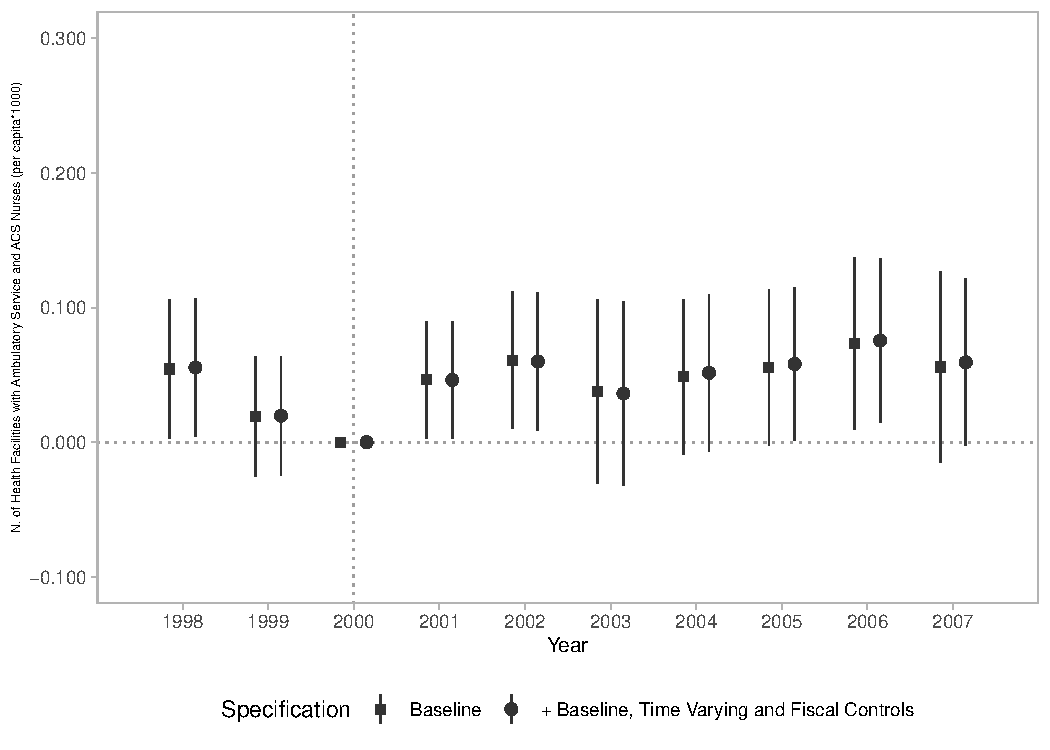
\includegraphics[width=\textwidth]{plots/sia_ncnes_enfacs_pcapita_dist_ec29_baseline_dist_ec29_baseline_12.pdf}
    \end{subfigure}
    \begin{subfigure}{0.32\textwidth}
        \centering
        \caption{\scriptsize Ambulatory Service and PSF Teams}\label{fig:12d}
        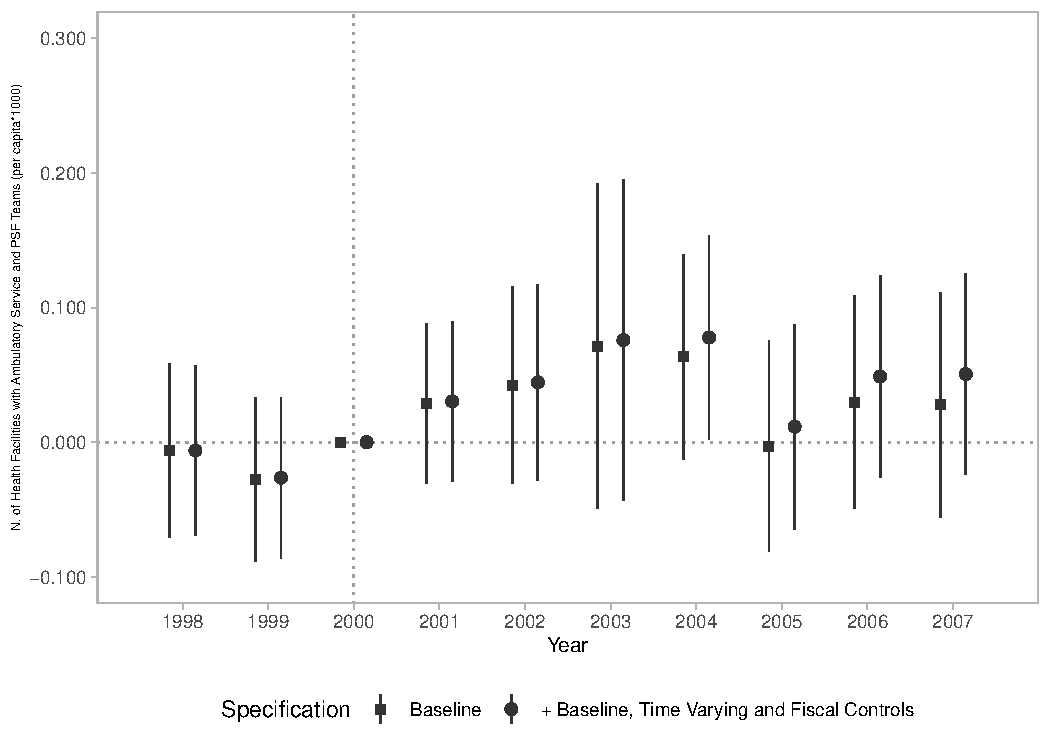
\includegraphics[width=\textwidth]{plots/sia_ncnes_psf_pcapita_dist_ec29_baseline_dist_ec29_baseline_12.pdf}
    \end{subfigure}
    \begin{subfigure}{0.32\textwidth}
        \centering
        \caption{\scriptsize Ambulatory Service and PSF Doctors}\label{fig:12e}
        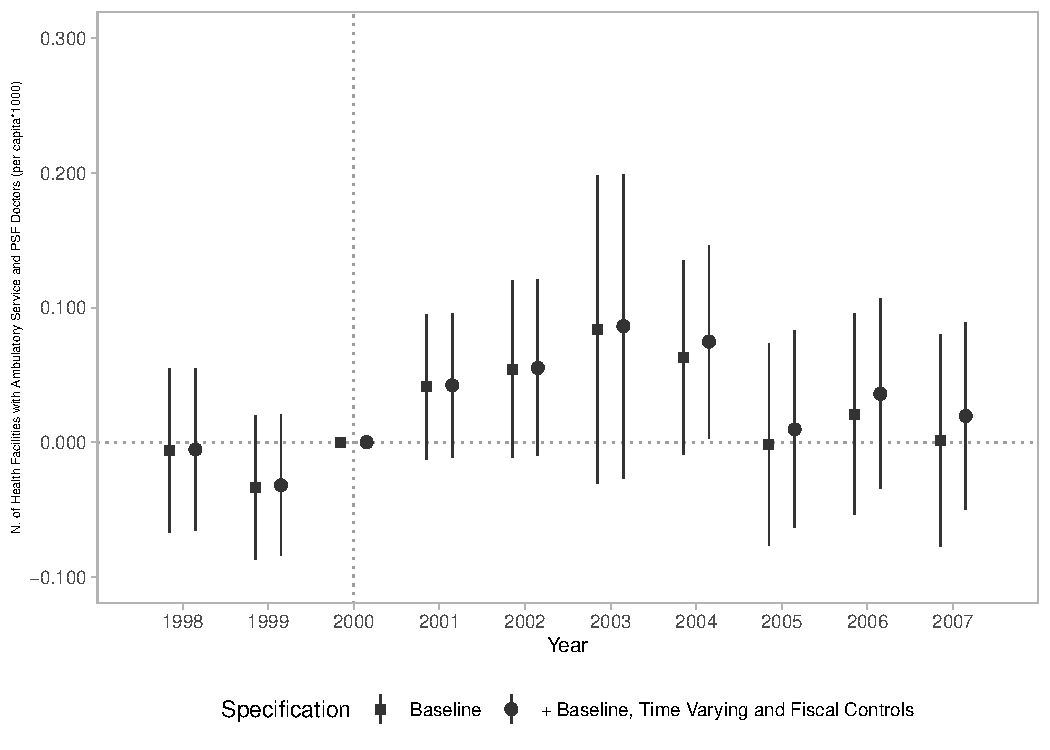
\includegraphics[width=\textwidth]{plots/sia_ncnes_medpsf_pcapita_dist_ec29_baseline_dist_ec29_baseline_12.pdf}
    \end{subfigure}
    \begin{subfigure}{0.32\textwidth}
        \centering
        \caption{\scriptsize Ambulatory Service and PSF Nurses}\label{fig:12f}
        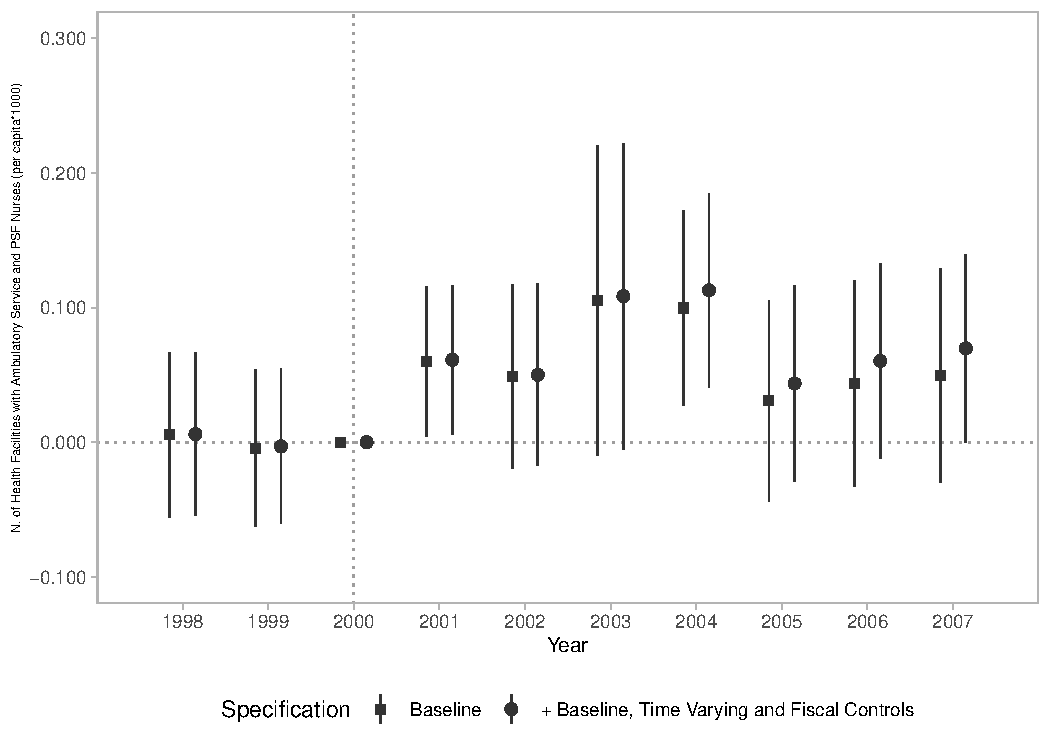
\includegraphics[width=\textwidth]{plots/sia_ncnes_enfpsf_pcapita_dist_ec29_baseline_dist_ec29_baseline_12.pdf}
    \end{subfigure}
        \begin{subfigure}{0.32\textwidth}
        \caption{\scriptsize Ambulatory Service and PSF Nursing Assistants}\label{fig:12g}
        \centering
        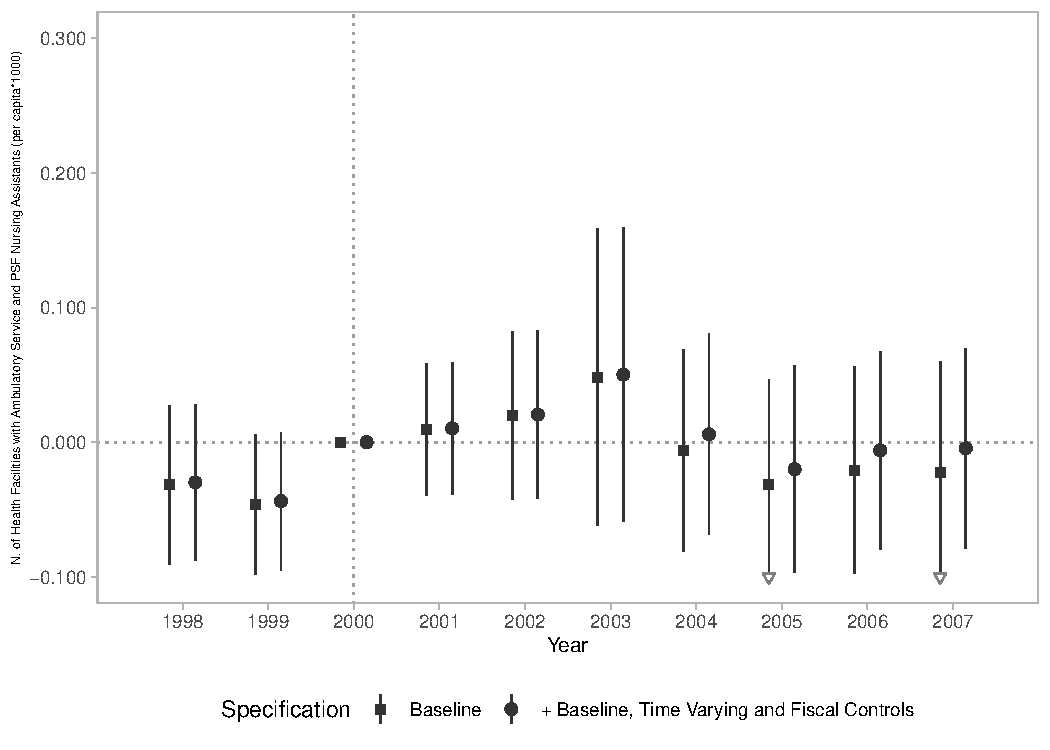
\includegraphics[width=\textwidth]{plots/sia_ncnes_outpsf_pcapita_dist_ec29_baseline_dist_ec29_baseline_12.pdf}
    \end{subfigure}

    
    \end{center}
    
                \scriptsize{Notes: The number of observations is 48916. DiD Estimates from Equation \ref{eq:2}. Independent variable is the distance to the EC/29 target in p.p. Square dots represent the baseline model with municipality and state-year fixed effects. Round dots represent fully saturated specification (Column 4 in regression Tables). Lines represent 95\% confidence intervals. Arrows, when present, indicate confidence intervals out of the plot bounds. Standard errors are clustered in the municipality level.}
    
\end{figure}